\documentclass[11pt]{article}

\usepackage[margin=1in]{geometry}
\usepackage[utf8]{inputenc}
\usepackage[T1]{fontenc}
\usepackage{hyperref}
\usepackage{url}
\usepackage{booktabs}
\usepackage{amsmath,amssymb}
\usepackage{graphicx}
\graphicspath{{plots/}}
\usepackage{subcaption}
\usepackage{microtype}
\usepackage{enumitem}
\usepackage{xcolor}

\title{Descriptor-Based Machine Learning for Redox Potential Prediction and Screening of Organic Quinone Cathode Candidates}

\author{
Vi Cheng, Harry Voorhis, Brian Donohugh\\
Stanford University\\
\texttt{vicheng@stanford.edu, hvoorhis@stanford.edu, bdono@stanford.edu}
}

\date{}

\begin{document}
\maketitle

\begin{abstract}
Organic redox-active molecules are promising candidates for next-generation battery cathodes, but identifying molecules with both high redox potential and acceptable gravimetric capacity is difficult. We study descriptor-based machine learning for predicting the redox potential (\texttt{deltaE\_V}) of 494 quinone molecules from 141 cleaned molecular descriptors. We compare Ridge regression, Random Forest, and a two-layer neural network (MLP) against physics-informed baselines built from frontier orbital descriptors (LUMO, HOMO). The MLP on the full descriptor set achieves test $R^2 = 0.924$ (95\% CI: [0.885, 0.951]) and RMSE $= 0.123$ V, compared with $R^2 = 0.848$ for Ridge and $R^2 = 0.787$ for Random Forest. Compact LUMO-only baselines still reach $R^2 = 0.648$, showing that frontier orbitals capture much of the signal. Descriptor-family ablations reveal that charge/E-state and hydrogen-bond-acceptor descriptors outperform frontier orbitals alone. Structural error analysis shows the model performs uniformly across molecule types. We embed the best predictor into a Pareto-based screening workflow combining predicted potential and theoretical capacity, producing a ranked candidate list.
\end{abstract}

\section{Introduction}

Electrochemical energy storage is important for electrified transportation and renewable-grid integration. Organic redox-active molecules offer chemical tunability and lower-cost synthesis compared to inorganic intercalation materials. Quinones are particularly interesting because small structural changes produce large shifts in redox behavior, making them natural targets for computational screening.

Selecting practical cathode candidates is multi-objective: a good candidate needs high redox potential (energy density), reasonable molecular weight (gravimetric capacity), and chemically plausible structural properties. DFT can estimate redox potentials but is too expensive for exhaustive screening, motivating ML surrogates that approximate redox behavior from precomputed molecular descriptors.

An important question is whether complex models add value over simple physics-based heuristics. Redox potential correlates strongly with frontier orbital energies (especially LUMO), so it is worth asking how much a full descriptor-based ML model improves over a compact LUMO-only baseline.

We study redox-potential prediction on a quinone dataset using Ridge regression, Random Forest, and a small neural network, comparing them against physics baselines of increasing complexity. We then analyze which descriptor families contribute most, perform structural error analysis, and connect prediction to a Pareto-style screening workflow. Our contributions are: (1) we quantify the gap between physics baselines and full ML models ($R^2 = 0.648$ vs.\ $0.924$); (2) we identify charge/E-state and H-bond-acceptor descriptors as the most informative families beyond frontier orbitals; (3) we analyze prediction errors by structural type; and (4) we demonstrate a multi-objective screening framework.

\section{Related Work}

Machine learning for molecular property prediction has grown rapidly, with models ranging from descriptor-based pipelines to graph neural networks \cite{butler2018, wu2018}. Descriptor-based approaches remain attractive on small datasets because they are data-efficient and interpretable, while nonlinear models can capture interactions that linear models miss \cite{gilmer2017}.

Organic redox-active molecules have been studied for battery and redox-flow applications. Er et al.\ \cite{er2014} screened quinones for redox flow batteries using DFT-derived properties. Hachmann et al.\ \cite{hachmann2011} demonstrated large-scale computational screening for organic photovoltaics. Ward et al.\ \cite{ward2018} developed a general-purpose ML framework for inorganic materials, showing that handcrafted features can compete with more complex representations. A recurring question is how much ML adds beyond simple electronic-structure proxies. Our work addresses this by benchmarking full ML models against compact frontier-orbital baselines and analyzing which descriptor families provide the largest marginal gains.

\section{Methods}

\subsection{Dataset and preprocessing}

We use a quinone-focused molecular dataset containing 494 molecules with 219 precomputed molecular descriptors and regression target \texttt{deltaE\_V} (redox potential in volts). The dataset includes pre-defined train/test splits (395/99), which we use as provided.

We remove non-numeric columns, zero-variance columns, and columns that are entirely missing. We drop one column from each pair with Pearson correlation $|r| > 0.95$, leaving 141 features. All filtering uses training data only. For Ridge and MLP, we standardize features using training-set statistics. Missing values are imputed with training-set column medians. We also construct a reduced set (\texttt{X\_reduced}) of the top 60 descriptors by correlation with the target.

\subsection{Physics baselines}

To separate domain knowledge from ML complexity, we define three compact baselines: \textbf{Phys-A} (LUMO only), \textbf{Phys-B} (LUMO + HOMO), and \textbf{Phys-C} (LUMO, HOMO, dipole moment, mean ionization energy, MAXDN2, MAXDN, min H-bond acceptor strength; 7 features). We fit linear and Ridge regression on each.

\subsection{Full ML models}

We compare three models on the full 141-feature matrix: \textbf{Ridge} ($\alpha \in \{10^{-4}, \ldots, 10\}$), \textbf{Random Forest} ($n_\text{est} \in \{100, 300\}$, depth $\in \{5, 10\}$, min leaf $\in \{1, 2\}$, features $= \sqrt{d}$), and \textbf{MLP} (input $\to$ 64/128 hidden $\to$ ReLU $\to$ dropout $\to$ output; Adam, 350 epochs; dropout $\in \{0, 0.1\}$, weight decay $\in \{10^{-5}, 10^{-4}\}$). All hyperparameters are selected by 5-fold CV maximizing $R^2$, retrained on full training data, and evaluated on the held-out test set with 95\% bootstrap CIs (1000 resamples).

\subsection{Ablation and error analysis}

We group descriptors into five families (frontier/electronic, H-bond acceptor, charge/E-state, topology/shape, size/mass/polarity) and train Ridge on each independently. We also analyze prediction errors by structural type: nitrogen content, aromaticity, ring count, and molecular weight group.

\subsection{Screening}

We estimate gravimetric capacity as $Q = nF / (3.6 \cdot MW)$ with $n = 2$ and $F = 96{,}485$ C/mol. We rank molecules by a weighted score (50\% normalized potential, 35\% normalized capacity, 15\% outlier penalty) and identify Pareto-optimal candidates.

\section{Results and Discussion}

\subsection{Model comparison}

Table~\ref{tab:results} summarizes the results. The MLP on the full descriptor set achieves test $R^2 = 0.924$ and RMSE $= 0.123$ V, outperforming Ridge ($R^2 = 0.848$) and Random Forest ($R^2 = 0.789$). The reduced feature set performs slightly worse across all models, confirming that the additional descriptors carry useful signal.

The physics baselines show that LUMO alone explains 65\% of the variance ($R^2 = 0.648$), and the 7-feature Phys-C reaches $R^2 = 0.729$. The progression from Phys-A to Phys-C to Ridge to MLP ($0.648 \to 0.729 \to 0.848 \to 0.924$) shows that each layer of complexity contributes. The Ridge-to-MLP jump ($+0.076$ in $R^2$) suggests that nonlinear descriptor interactions matter. The parity plot in Figure~\ref{fig:main_results}b confirms this: the MLP clusters more tightly around $y = x$, especially at higher potentials.

\begin{table}[t]
\centering
\caption{Test-set performance with 95\% bootstrap CIs (99 held-out molecules).}
\label{tab:results}
\small
\begin{tabular}{llccc}
\toprule
Model & Features & Test $R^2$ & RMSE (V) & MAE (V) \\
\midrule
MLP & X\_full (141) & \textbf{0.924} [0.885, 0.951] & \textbf{0.123} [0.100, 0.147] & \textbf{0.093} [0.078, 0.108] \\
Ridge & X\_full (141) & 0.848 [0.780, 0.897] & 0.173 [0.137, 0.210] & 0.121 [0.099, 0.147] \\
Rand.\ Forest & X\_full (141) & 0.789 [0.709, 0.859] & 0.204 [0.153, 0.259] & 0.137 [0.109, 0.171] \\
MLP & X\_red.\ (60) & 0.835 [0.769, 0.899] & 0.179 [0.130, 0.235] & 0.114 [0.089, 0.144] \\
\midrule
Linear Reg. & Phys-C (7) & 0.729 [0.574, 0.825] & 0.232 [0.188, 0.278] & 0.171 [0.143, 0.204] \\
Linear Reg. & Phys-B (2) & 0.668 [0.532, 0.759] & 0.256 [0.216, 0.299] & 0.194 [0.163, 0.229] \\
Linear Reg. & Phys-A (1) & 0.648 [0.520, 0.751] & 0.260 [0.221, 0.302] & 0.198 [0.166, 0.233] \\
\bottomrule
\end{tabular}
\end{table}

\begin{figure}[t]
    \centering
    \begin{subfigure}[b]{0.48\textwidth}
        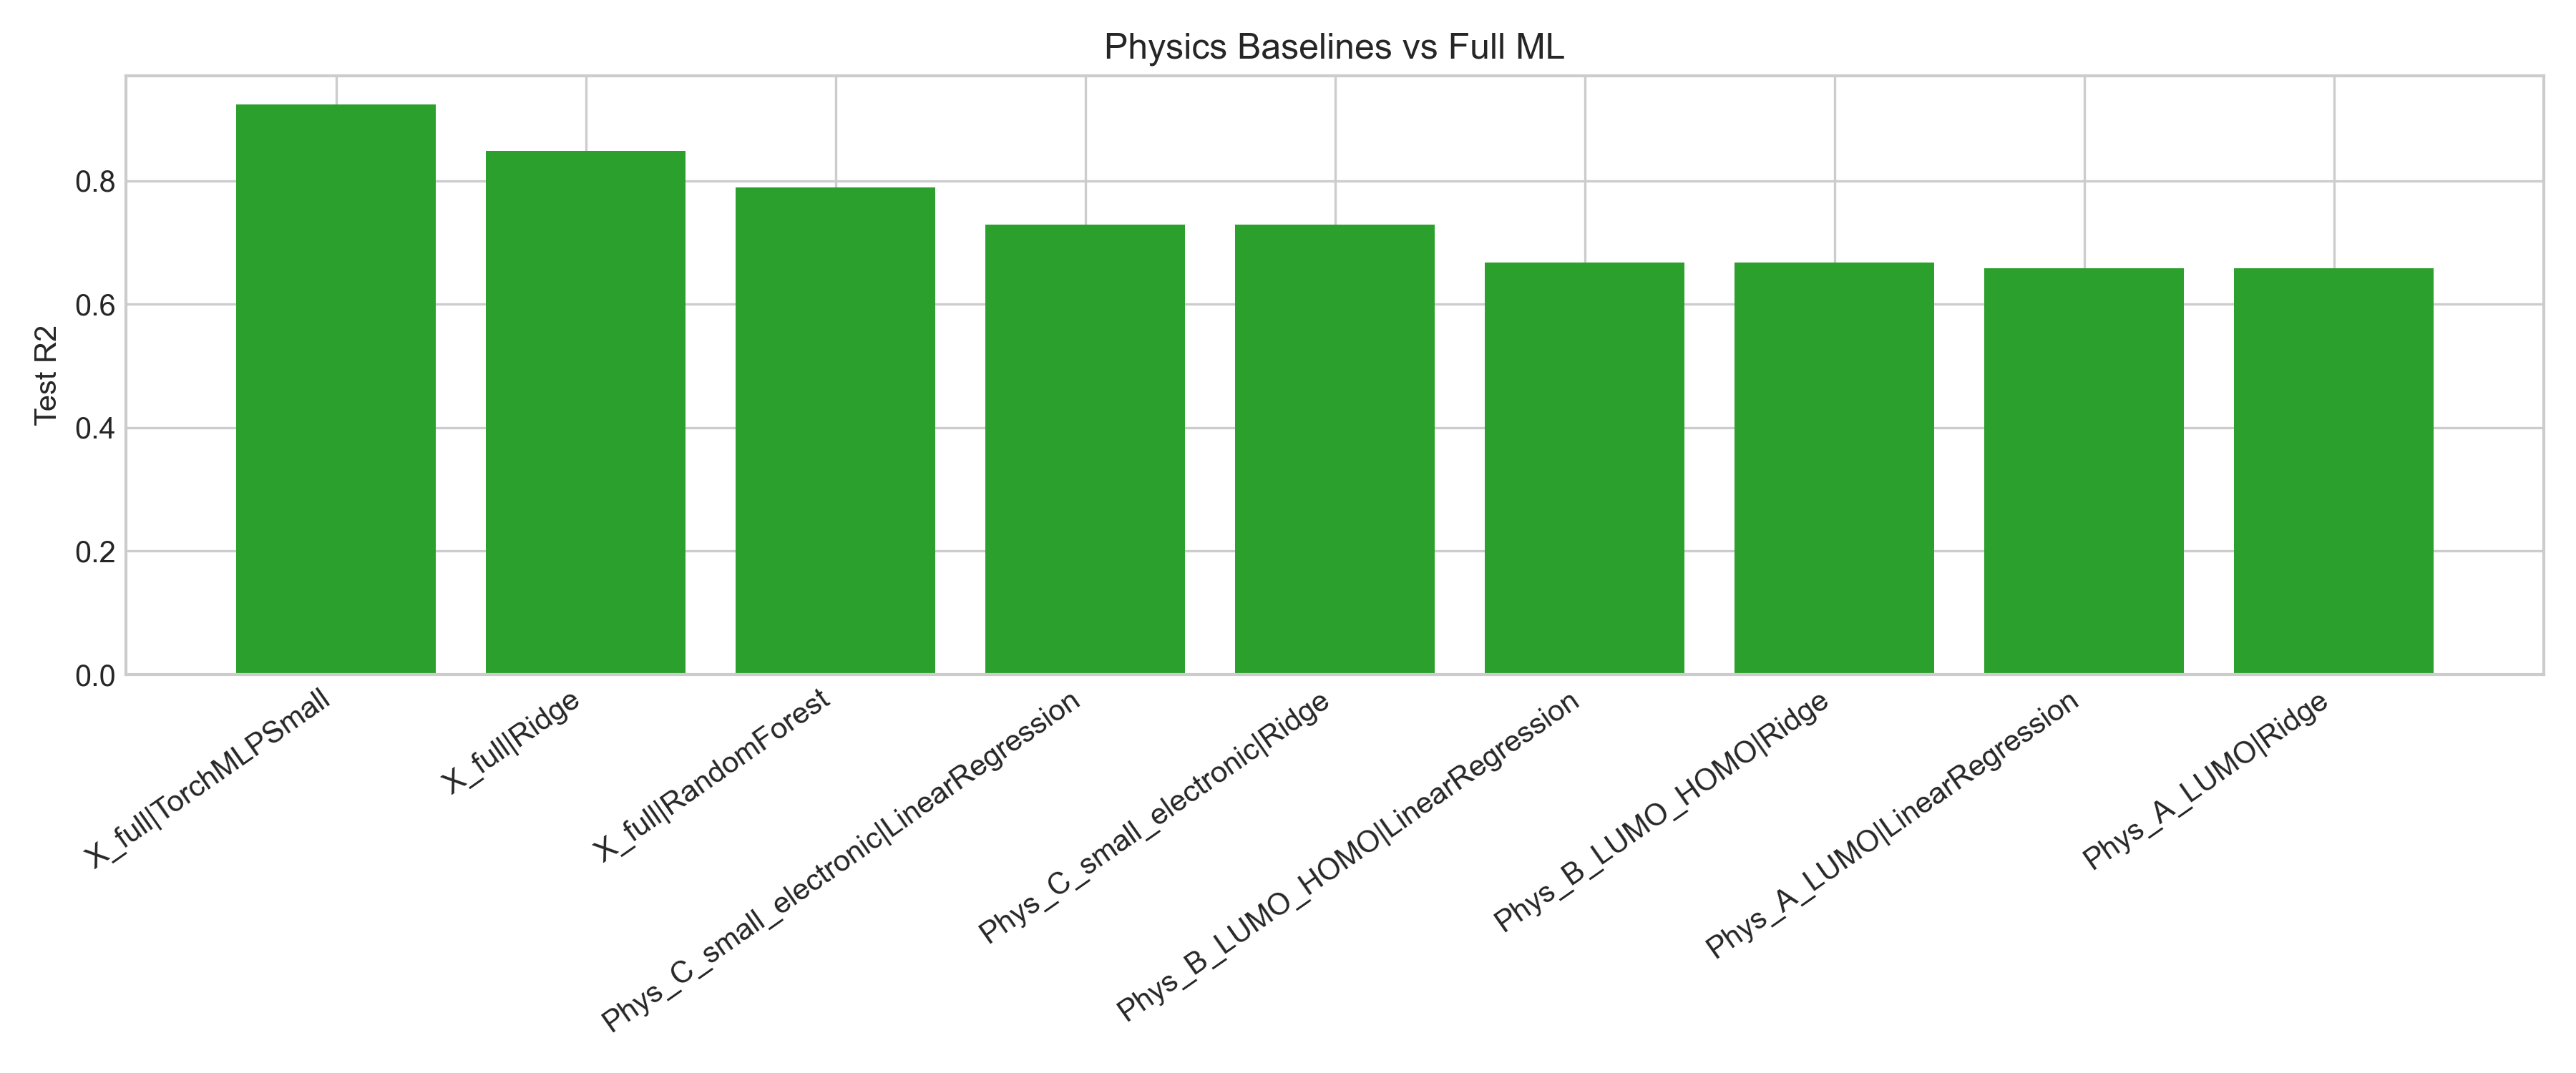
\includegraphics[width=\textwidth]{physics_vs_ml_r2.png}
        \caption{Test $R^2$ for physics baselines and full ML models.}
    \end{subfigure}
    \hfill
    \begin{subfigure}[b]{0.48\textwidth}
        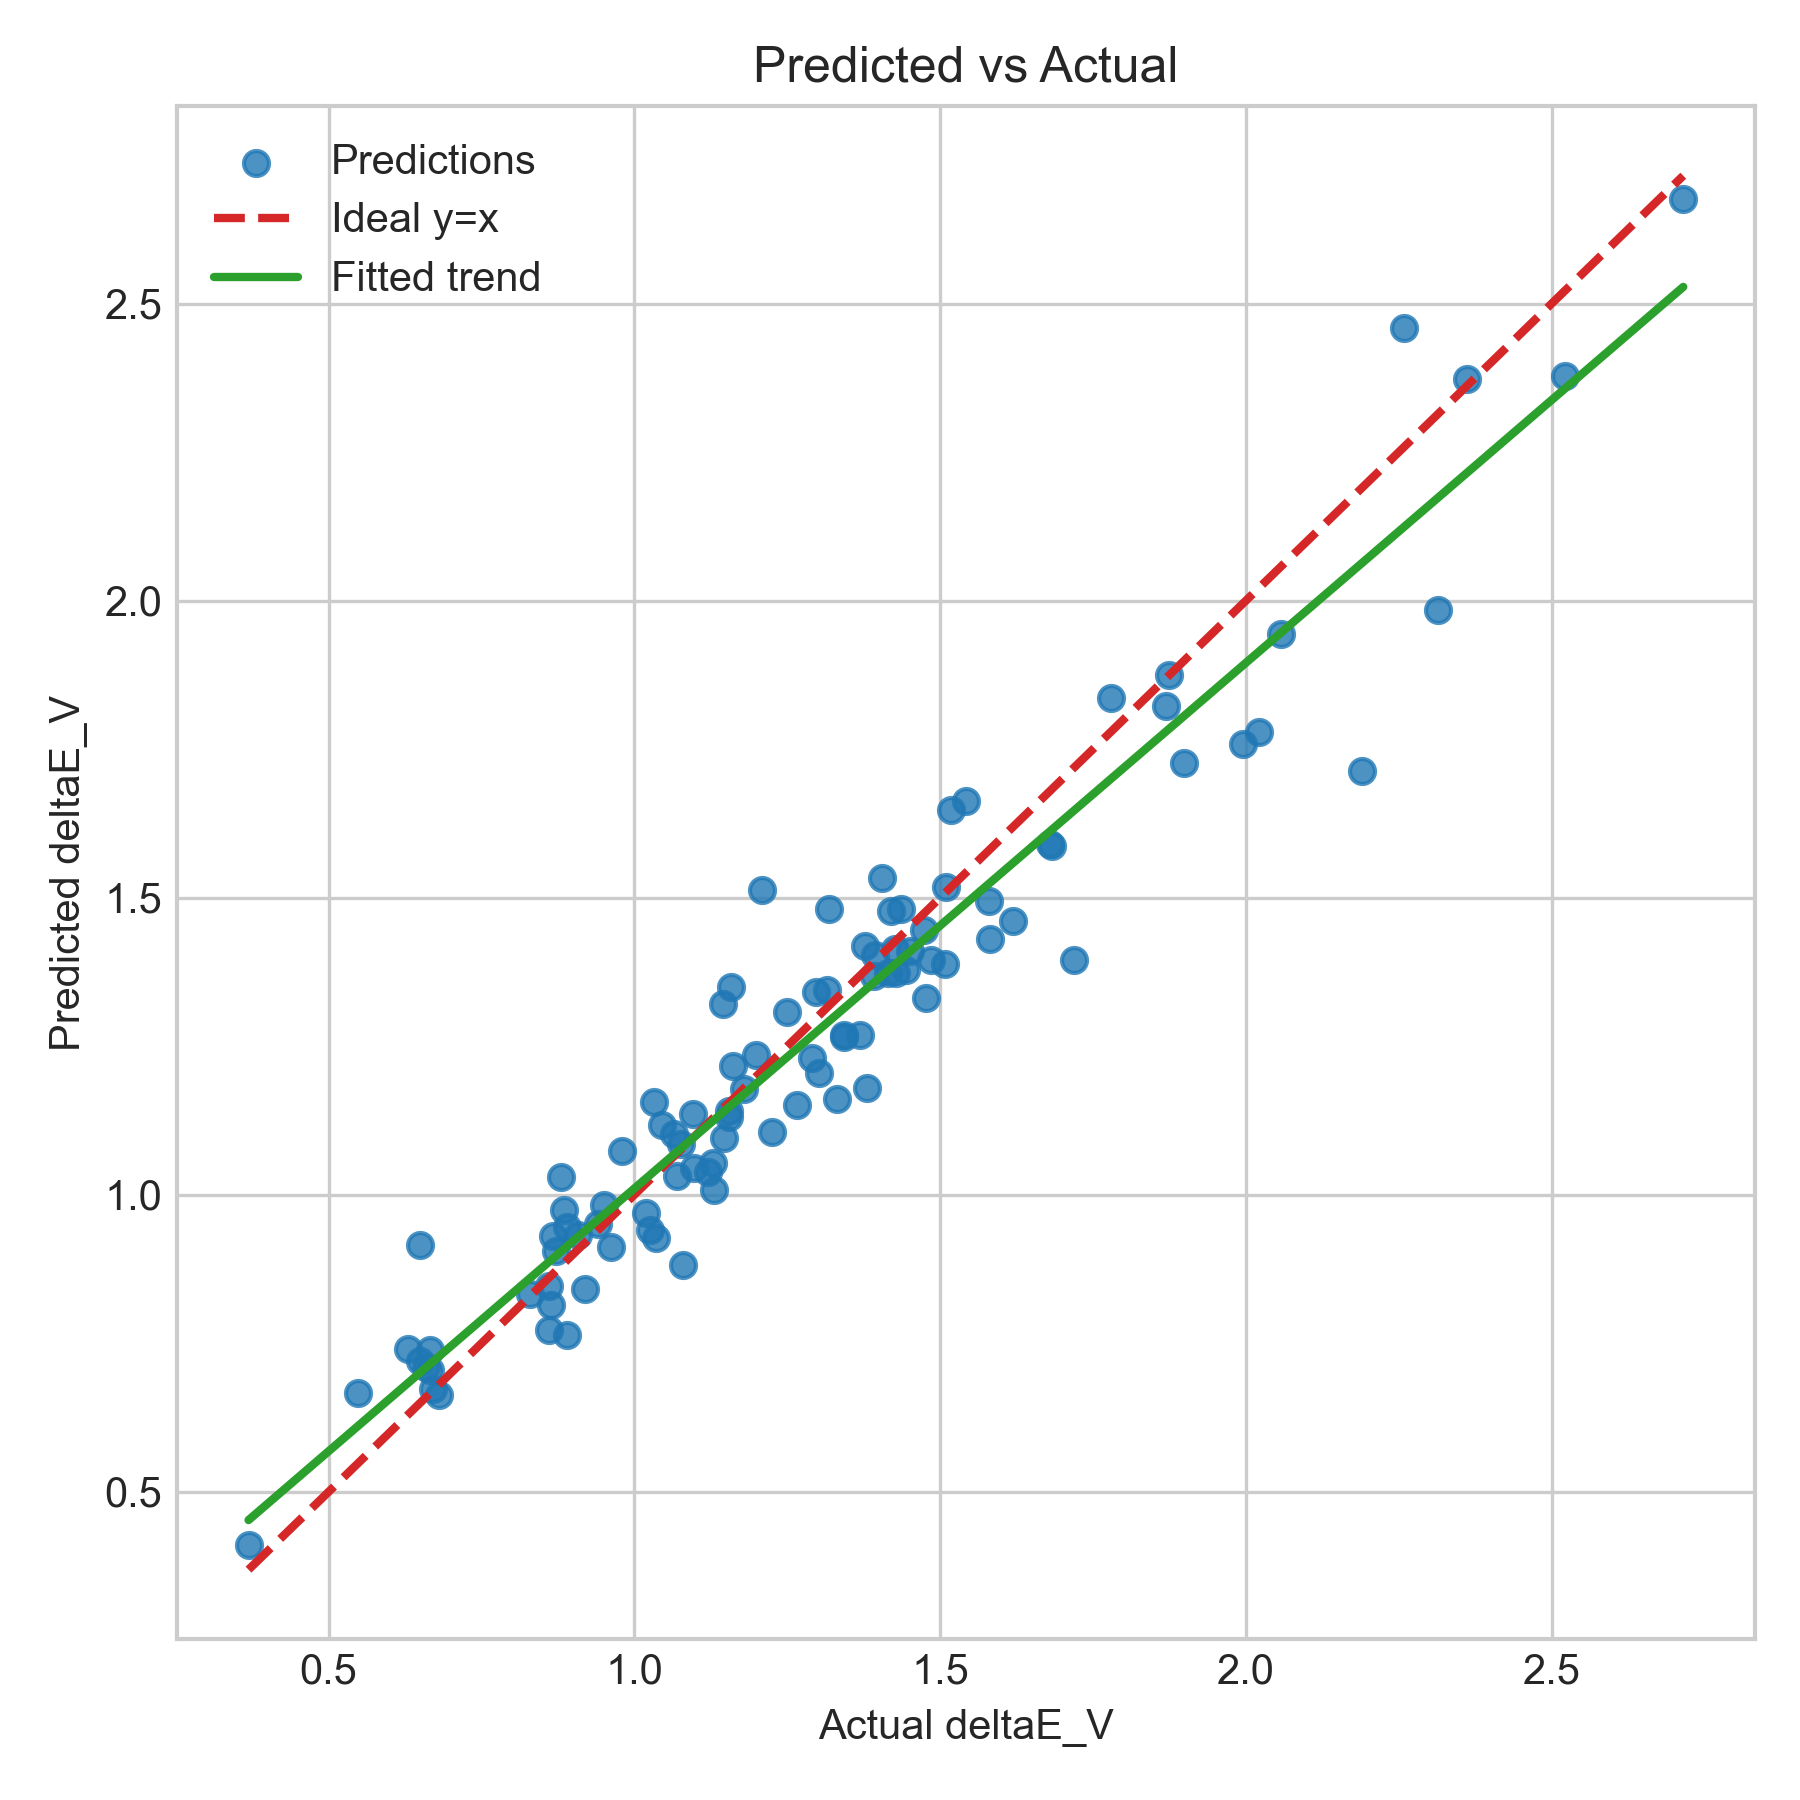
\includegraphics[width=\textwidth]{predicted_vs_actual.png}
        \caption{Predicted vs.\ actual for the best model (MLP, X\_full).}
    \end{subfigure}
    \caption{(a) Physics baselines vs.\ full ML models. (b) Parity plot for the MLP, with ideal $y = x$ in red.}
    \label{fig:main_results}
\end{figure}

\subsection{Descriptor-family ablations}

Figure~\ref{fig:ablations}a shows test $R^2$ when Ridge is trained on each descriptor family alone. Charge/E-state is strongest ($R^2 = 0.740$), followed by H-bond acceptor ($R^2 = 0.710$) and frontier/electronic ($R^2 = 0.679$). Topology/shape performs worst ($R^2 = 0.471$). The fact that charge/E-state outperforms the frontier/electronic family (which contains LUMO and HOMO) suggests that local charge distribution and electrotopological features encode redox-relevant information beyond global orbital energies. This aligns with the top individual correlations: LUMO ($|r| = 0.80$), \texttt{meanI} ($|r| = 0.75$), \texttt{minwHBa} ($|r| = 0.74$), and \texttt{MAXDN2} ($|r| = 0.72$).

\subsection{Structural error analysis}

We analyzed prediction errors of the best model grouped by structural properties of the test molecules. The model performs relatively uniformly: mean absolute error is 0.083 V for non-nitrogen-containing molecules vs.\ 0.099 V for nitrogen-containing ones; 0.079 V for aromatic molecules vs.\ 0.100 V for non-aromatic. By ring count, single-ring molecules show the highest error (MAE $= 0.118$ V) compared to two-ring (0.076 V) and three-ring (0.082 V). Error does not vary strongly with molecular weight. The largest outliers (up to 0.48 V) do not cluster in any single structural category, suggesting the model does not have a blind spot for a particular molecule type.

\subsection{Screening}

\begin{figure}[t]
    \centering
    \begin{subfigure}[b]{0.48\textwidth}
        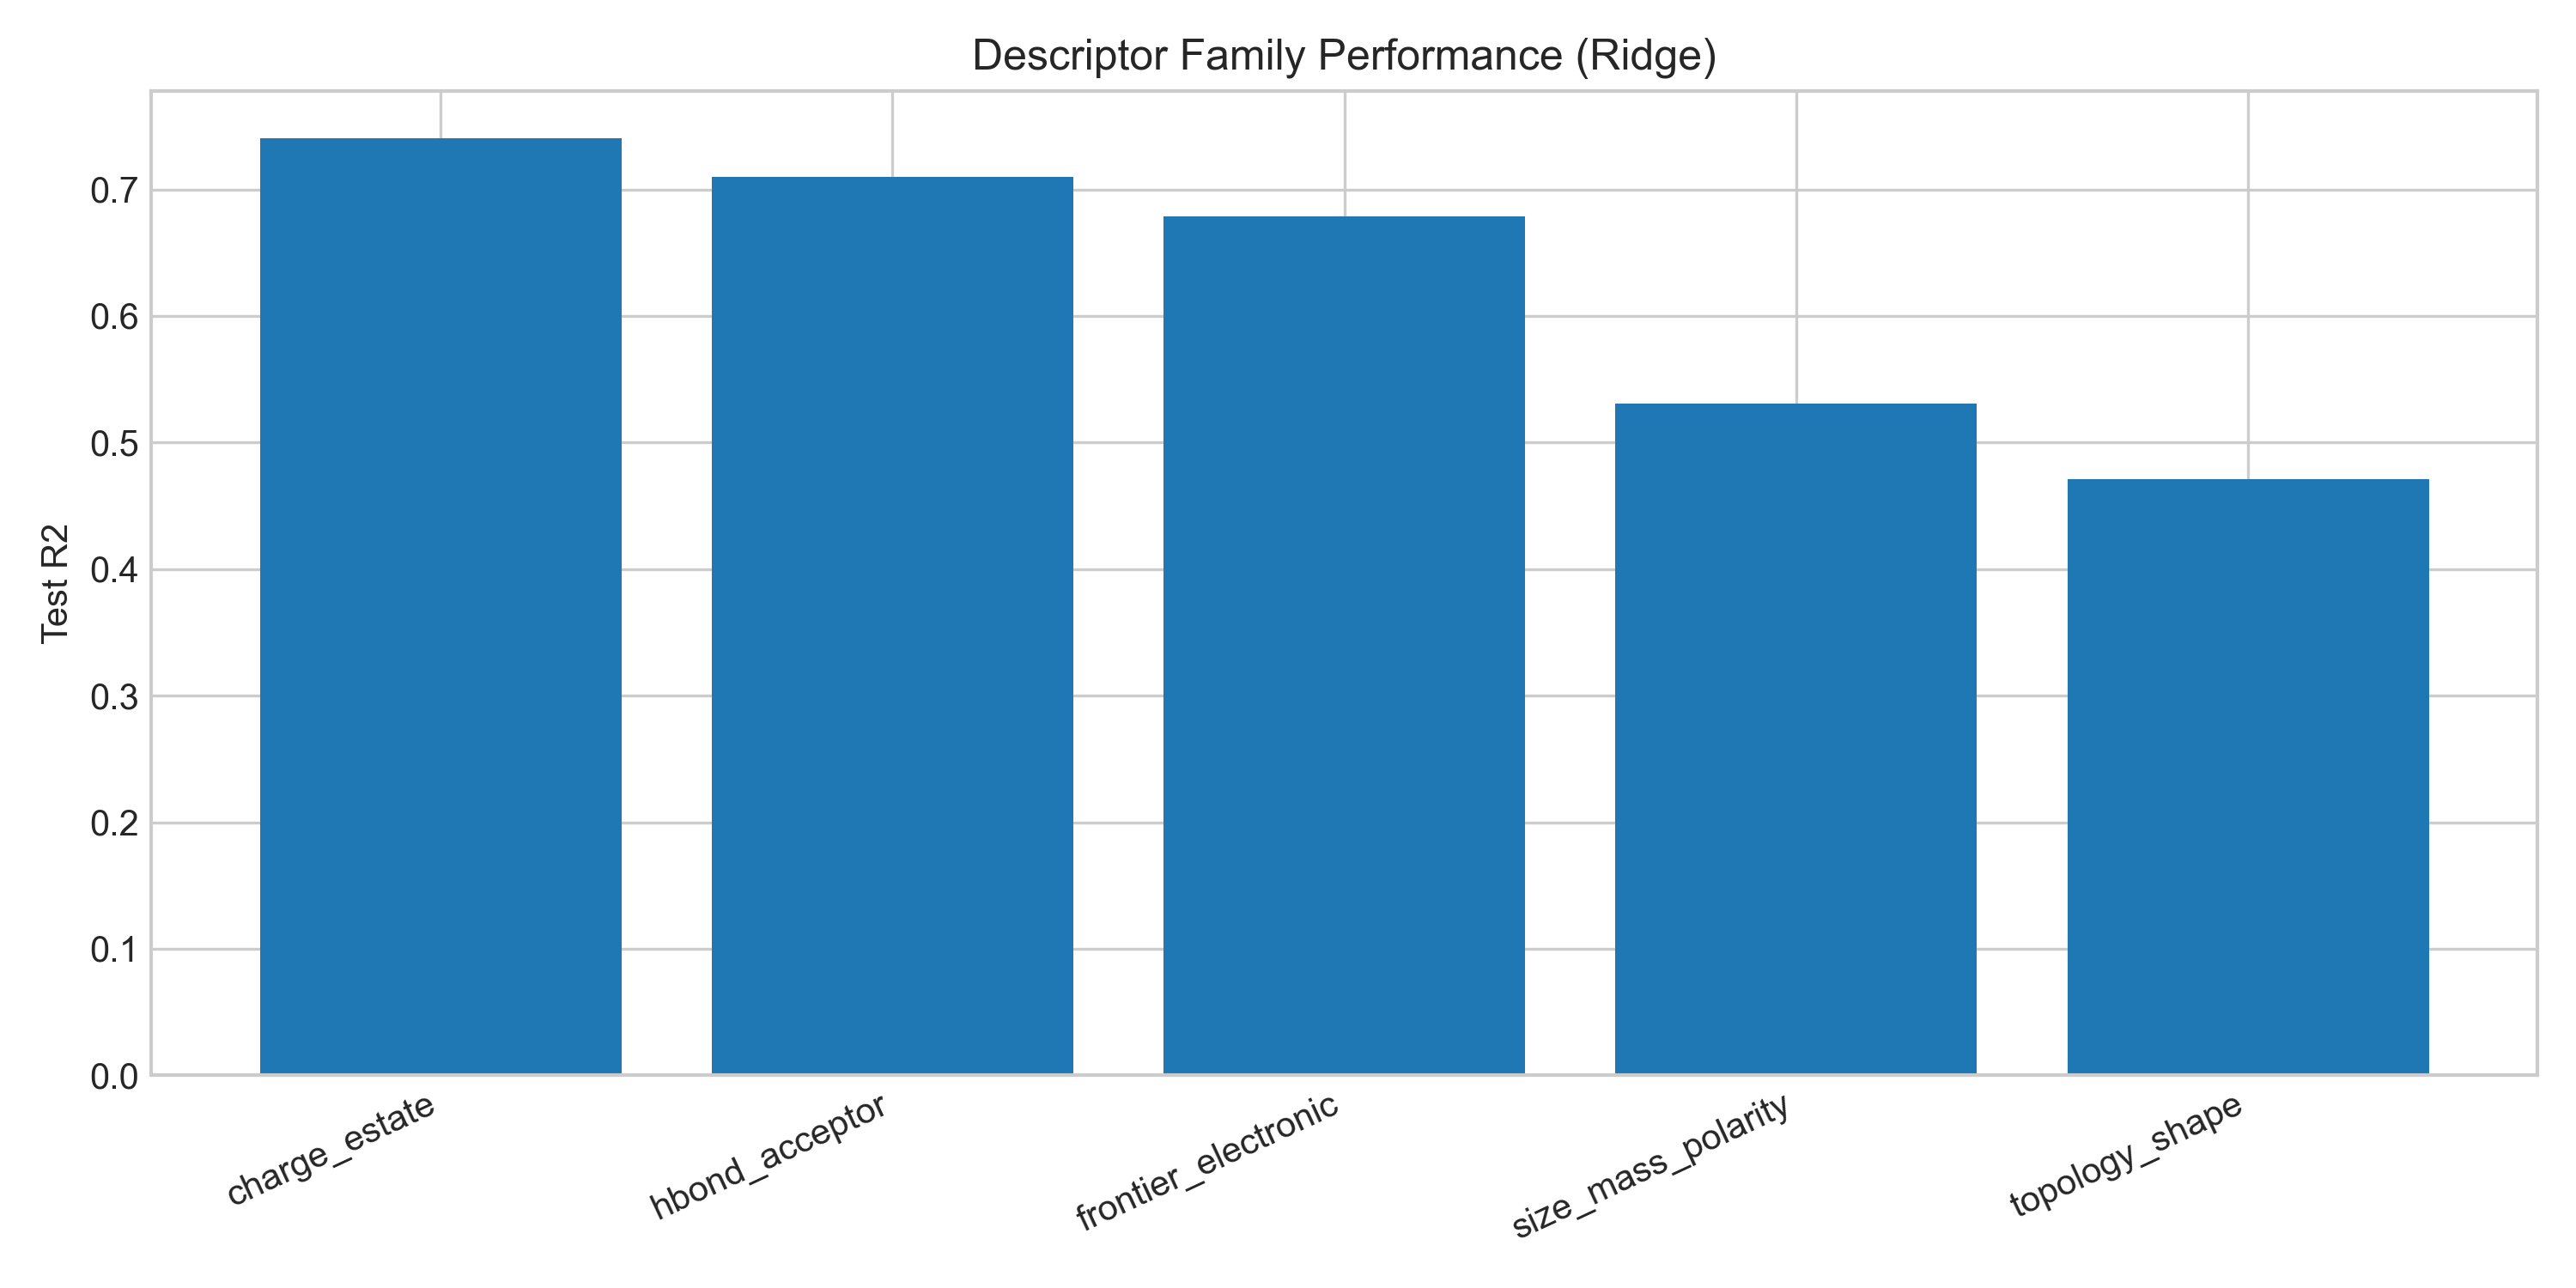
\includegraphics[width=\textwidth]{descriptor_family_performance.png}
        \caption{Descriptor-family test $R^2$ (Ridge).}
    \end{subfigure}
    \hfill
    \begin{subfigure}[b]{0.48\textwidth}
        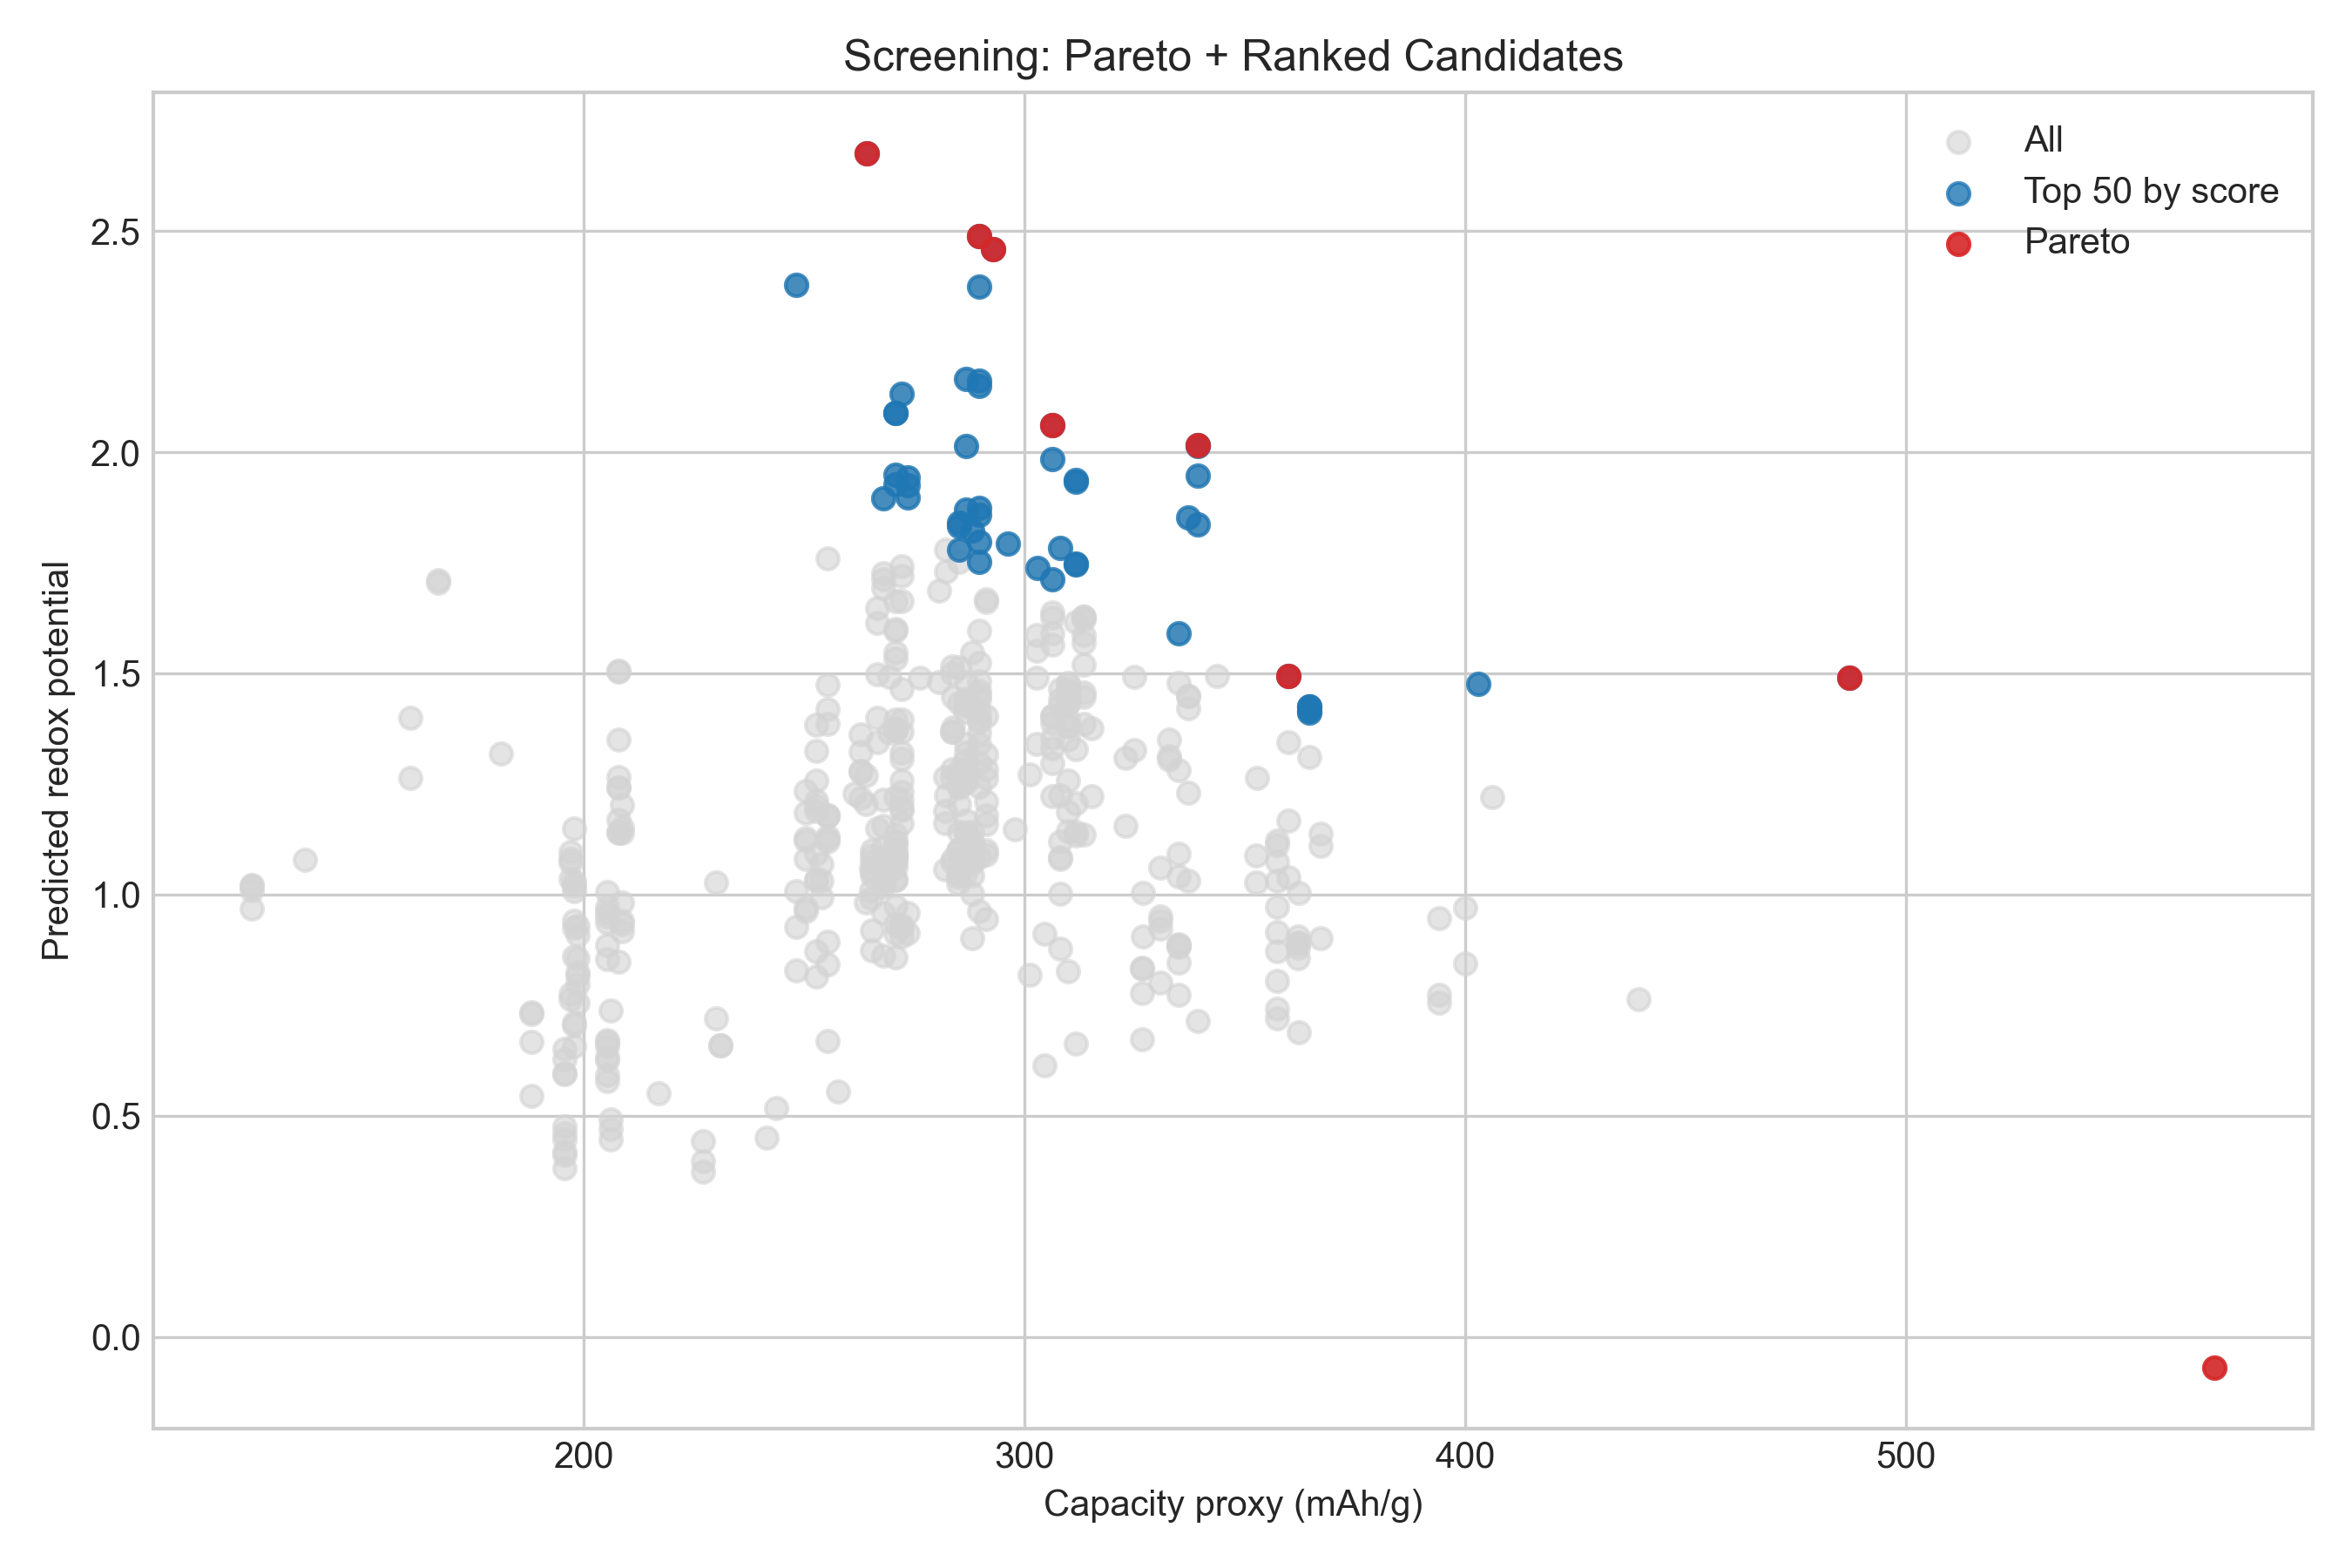
\includegraphics[width=\textwidth]{pareto_ranked_screening.png}
        \caption{Pareto screening: capacity vs.\ predicted potential.}
    \end{subfigure}
    \caption{(a) Charge/E-state descriptors are the most predictive single family. (b) Screening results with Pareto-optimal candidates in red and top-50 ranked in blue.}
    \label{fig:ablations}
\end{figure}

Figure~\ref{fig:ablations}b shows predicted redox potential against the capacity proxy for all 494 molecules, with Pareto-optimal candidates in red. The Pareto front reveals an explicit tradeoff: very high-potential molecules tend to have higher molecular weight (lower capacity). Top-ranked candidates cluster in the high-potential, moderate-capacity region. This two-objective view is more informative than sorting by potential alone. Full screening results are available in the code repository.

\subsection{Limitations}

With 99 test molecules, bootstrap CIs are relatively wide ($R^2$ CI spans ${\sim}0.07$ for the best model). The study uses precomputed descriptors rather than learned molecular representations; graph neural networks could potentially perform better on larger datasets. The screening weights (50/35/15) are heuristic and would benefit from domain-expert calibration.

\section{Conclusion}

We studied descriptor-based ML for predicting redox potentials of quinone molecules. A small MLP trained on 141 descriptors achieves $R^2 = 0.924$ on a held-out test set, substantially outperforming linear models and compact frontier-orbital baselines. LUMO alone reaches $R^2 = 0.648$, showing that frontier orbitals capture much of the signal, but the full model closes most of the remaining gap. Descriptor-family ablations show that charge/E-state and H-bond-acceptor features contribute the most. Structural error analysis confirms that model accuracy is consistent across molecule types. We also demonstrated a Pareto-based screening workflow combining predicted potential and gravimetric capacity.

Future work could incorporate graph-based molecular representations, test on more chemically diverse datasets, and add solubility and stability criteria to the screening framework.

\begin{thebibliography}{9}

\bibitem{butler2018}
K.~T. Butler, D.~W. Davies, H.~Cartwright, O.~Isayev, and A.~Walsh.
Machine learning for molecular and materials science.
{\em Nature}, 559:547--555, 2018.

\bibitem{wu2018}
Z.~Wu, B.~Ramsundar, E.~N. Feinberg, J.~Gomes, C.~Geniesse, A.~S. Pappu, K.~Leswing, and V.~Pande.
MoleculeNet: A benchmark for molecular machine learning.
{\em Chemical Science}, 9:513--530, 2018.

\bibitem{gilmer2017}
J.~Gilmer, S.~S. Schoenholz, P.~F. Riley, O.~Vinyals, and G.~E. Dahl.
Neural message passing for quantum chemistry.
In {\em Proc.\ ICML}, 2017.

\bibitem{er2014}
S.~Er, C.~Suh, M.~P. Marshak, and A.~Aspuru-Guzik.
Computational design of molecules for an all-quinone redox flow battery.
{\em Energy Environ.\ Sci.}, 8:3024--3027, 2015.

\bibitem{hachmann2011}
J.~Hachmann, R.~Olivares-Amaya, S.~Jinich, et al.
The Harvard Clean Energy Project: Large-scale computational screening and design of organic photovoltaics on the world community grid.
{\em J.\ Phys.\ Chem.\ Lett.}, 2:2241--2251, 2011.

\bibitem{ward2018}
L.~Ward, A.~Agrawal, A.~Choudhary, and C.~Wolverton.
A general-purpose machine learning framework for predicting properties of inorganic materials.
{\em npj Comput.\ Mater.}, 2:16028, 2016.

\end{thebibliography}

\end{document}
